 \documentclass[xcolor=dvipsnames, aspectratio=169, 10pt]{beamer}
% \usepackage{vntex}
\usetheme[sectionpage=progressbar,subsectionpage=progressbar]{metropolis}
\usepackage{tikz}
\usetikzlibrary{bayesnet}
\usetikzlibrary{arrows}
\usetikzlibrary{backgrounds}
\usepackage{caption}
\usepackage{animate}
\usepackage{bm}
% \setbeamertemplate{caption}[numbered]
% \usepackage{subcaption}

\usepackage[lined,commentsnumbered]{algorithm2e}
\beamertemplatenavigationsymbolsempty
% \useinnertheme{circles}
%\useoutertheme{split}

\definecolor{background}{HTML}{274150}
\definecolor{sbackground}{HTML}{b51823}
\definecolor{main-text}{HTML}{80A07C}
\definecolor{enumercolor}{HTML}{A4CCE0}
\definecolor{progress-bar}{HTML}{E6CBA0}\usecolortheme[named=sbackground]{structure} % define for item color, commented Jan 4,2024

%% TITLE PAGE 
\title[]{TASK SCHEDULING USING RECURRENT NEURAL NETWORKS AND DEEP REINFORCEMENT LEARNING}
\subtitle{Deep Learning Project}

\AtBeginDocument{
	\author[Minh]{
		\begin{tabular}{lll}
			\textit{\small Supervisor:} & \small Dr. Achille Mbogol Touye \\
			\textit{\small Student:} & \small CHAU Dang Minh
            \vspace{.5cm}\\
		\end{tabular}
	}
}
\institute[Limoges]{
	{
		University of Limoges
	}
}
% TOC
\setbeamertemplate{section in toc}[circle]
\setbeamercolor{section in toc}{bg=sbackground!40, fg=black} % change color section item
 \setbeamerfont{section number projected}{size=\large}
% ENUM
  % \setbeamercolor{item projected}{bg=red!70!black,fg=white}
  \setbeamercolor{frametitle}{fg=sbackground,bg=sbackground!40} % change color bar
  \setbeamercolor{background canvas}{bg=white} % change color frame
  \setbeamercolor{normal text}{fg=black} % change text color
\setbeamercolor{progress bar}{fg=progress-bar!110,bg=progress-bar!50} % change progress bar color
    \setbeamertemplate{enumerate items}[circle]
    \setbeamerfont{itemize item projected}{size=\huge}
        \setbeamerfont{item projected}{size=\large}
% CAPTION
\setbeamertemplate{caption}{\raggedright\insertcaption\par}
% LOGO
\usepackage{textpos} 

\addtobeamertemplate{frametitle}{}{%
	\begin{textblock*}{100mm}(\textwidth,-.9cm)
		% 
\includegraphics[height=.7cm,width=.7cm]{logo.png}
\end{textblock*}}
\usepackage{eso-pic}
\usepackage{pgf}
\titlegraphic{
	\begin{picture}(0,0)
		\put(420,5){\makebox(0,0)[rt]{
\includegraphics[width=3cm]{logo.png}}}
	\end{picture}
}
\setbeamertemplate{bibliography item}{\insertbiblabel}
\newcommand{\nologo}{\setbeamertemplate{logo}{}}
% HEADLINE
%\setbeamertemplate{headline}{}
% FOOTLINE
\setbeamercolor{custom1}{fg=black,bg=mycolor}
\setbeamercolor{custom2}{fg=black, }
\setbeamercolor{custom3}{fg=black,}
\setbeamerfont{footline}{series=\bfseries}%, family=\ttfamily}
\setbeamertemplate{footline}{%
	\leavevmode%
% 	\begin{beamercolorbox}[wd=0.25\textwidth, sep=0.4em, center]{custom1}%
% 		\strut \quad\insertshortauthor \quad (\insertshortinstitute)
% 	\end{beamercolorbox}%
% 	\begin{beamercolorbox}[wd=0.45\textwidth, sep=0.4em, center]{custom2}%
% 		\strut \insertshorttitle
% 	\end{beamercolorbox}%
	\begin{beamercolorbox}[wd=1\textwidth, sep=0.4em, right]{custom3}%
		\strut \insertframenumber/\inserttotalframenumber
	\end{beamercolorbox}%
}
% Thank you slide
\makeatletter
\let\beamer@writeslidentry@miniframeson=\beamer@writeslidentry%
\def\beamer@writeslidentry@miniframesoff{%
	\expandafter\beamer@ifempty\expandafter{\beamer@framestartpage}{}% does not happen normally
	{%else
		% removed \addtocontents commands
		\clearpage\beamer@notesactions%
	}
}
\newcommand*{\miniframeson}{\let\beamer@writeslidentry=\beamer@writeslidentry@miniframeson}
\newcommand*{\miniframesoff}{\let\beamer@writeslidentry=\beamer@writeslidentry@miniframesoff}
\makeatother
% COMMAND
\newcommand\norm[1]{\left\lVert#1\right\rVert}
\newcommand\sym{\mathcal{S}}

\newcommand{\scrP}{\mathscr{P}}
% Remove main reference numbering
\setbeamertemplate{frametitle continuation}{}

% Command for some notations
\newcommand{\prob}[1]{\text{p}({#1})}
\newcommand{\expect}[1]{\mathbb{E}({#1})}
\newcommand{\im}[1]{\text{Im}({#1})}
\newcommand{\var}[1]{\text{V}({#1})}
\newcommand{\normal}[2]{\mathcal{N}({#1}, {#2})}

\newcommand{\Pib}{\boldsymbol{\Pi}}
\newcommand{\Alphab}{\boldsymbol{\Alpha}}
\newcommand{\Betab}{\boldsymbol{\Beta}}
\newcommand{\Thetab}{\boldsymbol{\Theta}}
\newcommand{\Etab}{\boldsymbol{\Eta}}
\newcommand{\Lambdab}{\boldsymbol{\Lambda}}
% \addbibresource{refs.bib}

\newcommand{\Zb}{\mathbf{Z}}
\newcommand{\Xb}{\mathbf{X}}
\newcommand{\Wb}{\mathbf{W}}
\newcommand{\KL}{\text{KL}}
% DOCUMENT
\begin{document}
\date{}
\captionsetup[figure]{labelformat=empty, font={footnotesize,it}}
\begin{frame}[noframenumbering,plain]
    \titlepage
\end{frame}

\begin{frame}
    \frametitle{Outline}
    \tableofcontents
\end{frame}
\section{Introduction}

\begin{frame}{Scenerio}
  \begin{equation}
    \min\limits_{x\in \X} f(x),
  \end{equation}
  where
  \begin{itemize}
    \item $\X\in\RR^d$ is a closed convex set,
    \item $f:\X\to\RR$ is a continuously differentiable convex.
  \end{itemize}
  We use the standard Euclidean norm $\|x\|= \dfrac{1}{2}\langle x,x\rangle$.
  function
\end{frame}

\begin{frame}{Discreteness and Continuality}
  \begin{itemize}
    \item Early iterative optimization algorithms (Gradient Descent and Polyak's Momentum Acceleration) are intuitively interpretable.
    \item Nesterov's Acceleration is less intuitive
          \begin{equation}
            \begin{cases}
              x_k = y_{k-1} - s\nabla f(y_{k-1}) \\
              y_k = x_k + \dfrac{k-1}{k+2}(x_k - x_{k-1}).
            \end{cases}
          \end{equation}
    \item Continualized versions as ODEs are available.
    \item Current orientation: starting from an ODE and derive a family of discrete algorithms using Euler's methods.
  \end{itemize}
\end{frame}

\begin{frame}{Lagrangian mechanics and the Lagrangian}
  The Lagrangian $\L(X,V,t)$ is introduced \footnote{Wibisono, Andre, Ashia C. Wilson, and Michael I. Jordan. "A variational perspective on accelerated methods in optimization." proceedings of the National Academy of Sciences 113.47 (2016): E7351-E7358.} as a framework to derive ODEs, where
  \begin{itemize}
    \item $X = X(t)$ is the coordinate
    \item $V = \dot{X}(t)$ is the velocity
    \item $t\in\RR$ is the time
  \end{itemize}

  The action in $[t_1, t_2]$ is $\A(X) = \int\limits_{t_1}^{t_2} \L(X,V,t)\,\mathrm{d}t$. A trajectory $X$ being a stationary function of $\A$ solves the Euler-Lagrange equation
  \begin{equation}
    \dfrac{\partial \L}{\partial X} \L (X, V, t) = \dfrac{\mathrm{d}}{\mathrm{d}t} \dfrac{\partial \L}{\partial V} \L (X, V, t).
  \end{equation}
\end{frame}

\begin{frame}{NAG's Lagrangian}
  The ODE associated to NAG \footnote{Su, Weijie, Stephen Boyd, and Emmanuel J. Candes. "A differential equation for modeling Nesterov's accelerated gradient method: theory and insights." arXiv preprint arXiv:1503.01243 (2015).}
  \begin{equation}
    \label{eq:nes-ode}
    \ddot{X} + \dfrac{3}{t}\dot{X} + \nabla f(X) = 0
  \end{equation}
  has corresponding Lagrangian
  \begin{equation}
    \label{eq:nes-lagrangian}
    \L (X, V, t) = t^3\left(\dfrac{1}{2}\|V\|^2-f(X)\right).
  \end{equation}
  Indeed, $\dfrac{\partial \L}{\partial X} \L = -t^3\nabla f(X), \dfrac{\partial \L}{\partial V} \L = t^3V$ and $\dfrac{\mathrm{d}}{\mathrm{d}t}\dfrac{\partial \L}{\partial V} \L = 3t^2 V + t^3\dot{V}.$

  Hence $t^3\dot{X} = 3t^2\dot{X} + t^3\ddot{X}$. Divide by $t^3$ and rearrange to get (\ref{eq:nes-ode}).
\end{frame}

\begin{frame}{Lagrangian}
  \begin{itemize}
    \item We can also see that the standard Lagrangian
          \begin{equation}
            \label{eq:standard-lagrangian}
            \L (X, V, t) = \dfrac{1}{2}\|V\|^2-f(X)
          \end{equation}
          derives Polyak's acceleration with momentum $\beta=1$.
    \item In (\ref{eq:standard-lagrangian}), $\dfrac{1}{2}\|V\|^2$ is the kinetic energy and $f(X)$ is the potential energy.
    \item Idea: generalizing this difference, proving convergence of the derived ODE, then discretizing and proving the convergence of iterative algorithms.
  \end{itemize}
\end{frame}
\section{Dataset}
\setcounter{footnote}{1}

\begin{frame}{Dataset}
    \begin{itemize}
        \item MIT Supercloud Dataset \footnotetext{https://www.kaggle.com/datasets/skylarkphantom/mit-datacenter-challenge-data}
        \item One-year HPC task record
        \item Concerning features: \texttt{time\_submit}, \texttt{time\_start}, \texttt{time\_end}, \texttt{nodes\_alloc}
    \end{itemize}
\end{frame}

\begin{frame}{Dataset Processing}
    \begin{itemize}
        \item Assumption: all nodes have the same computing capacity
        \item Introduce $\texttt{task\_complexity} = (\texttt{time\_end} - \texttt{time\_start}) \times \texttt{nodes\_alloc}$
        \item Train and test data contain \texttt{time\_submit} and \texttt{task\_complexity}.
        \item Due to computation limit, secondly and minutely predictions are intractable. Daily prediction cannot capture patterns. As an experiment, we group complexities by hour.
        \item Dataset is split into $90\%$ for training and $10\%$ for testing.
    \end{itemize}
\end{frame}

\begin{frame}{Dataset Processing}
    \begin{figure}
        \centering
        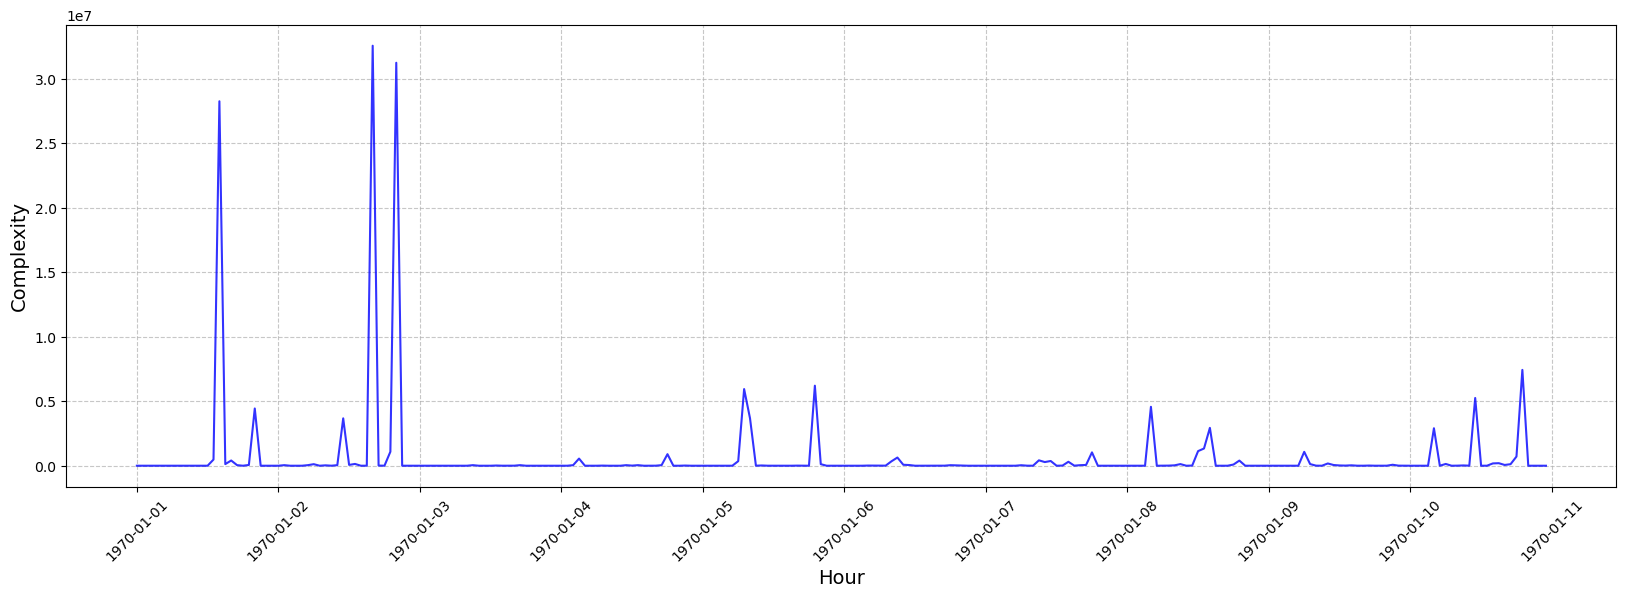
\includegraphics[width=0.8\linewidth]{img/hourly_complexity.png}
        \caption{Task complexity grouped by hour}
    \end{figure}
\end{frame}

\begin{frame}{Dataset Processing}
    \begin{figure}
        \centering
        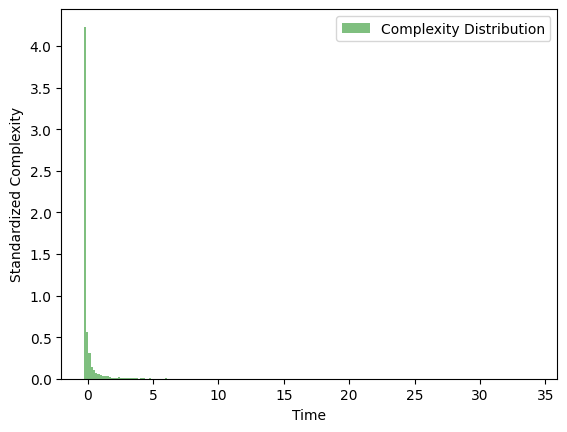
\includegraphics[width=0.7\linewidth]{img/task_complexity_distribution.png}
        \caption{High skewness of task complexity distribution}
    \end{figure}
\end{frame}


\section{Approaches}
\subsection{Recurrent Neural Networks}

\begin{frame}{Preparation}
    \begin{enumerate}
        \item Fill all time stamps with no task with a complexity-free task
        \item Train a recurrent neural network (GRU or LSTM) to predict task complexity in the next time stamp
        \item Store the trained task complexity distribution to decide the number of allocated nodes. Suppose that a task with complexity $C$ is at cumulative distribution point $p$, then it is allocated
              $$\min\{\texttt{available\_nodes}, \texttt{total\_nodes}\times p\}.$$
    \end{enumerate}
\end{frame}

\begin{frame}{Training and Testing}
    We train a two-layer LSTM with a 64-dimensional fully connected layers during 300 epochs.
    \begin{figure}
        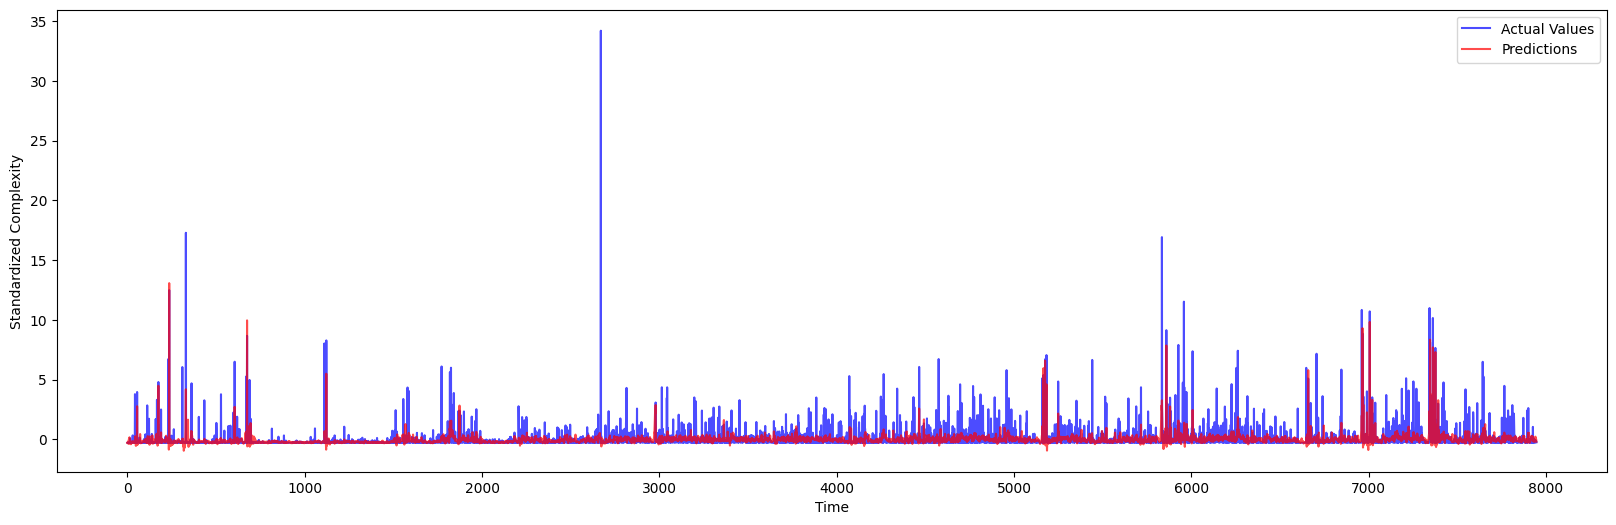
\includegraphics[width=0.9\textwidth]{img/train_accuracy.png}
        \caption{Model fit on the training data}
    \end{figure}
\end{frame}

\begin{frame}{Recurrent Neural Networks}
    \begin{figure}
        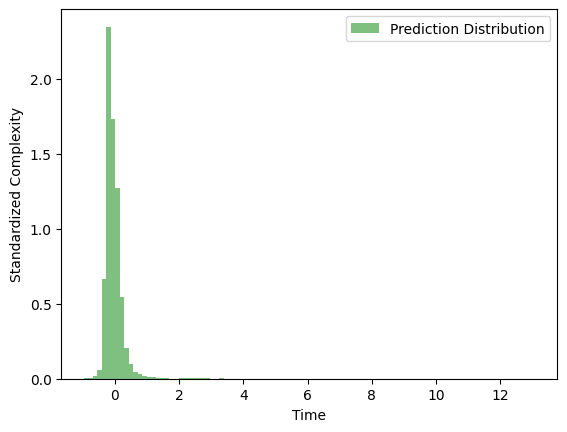
\includegraphics[width=0.5\textwidth]{img/complexity_ditribution.png}
        \caption{Complexity distribution}
    \end{figure}
\end{frame}

\begin{frame}{Recurrent Neural Networks}
    \begin{figure}
        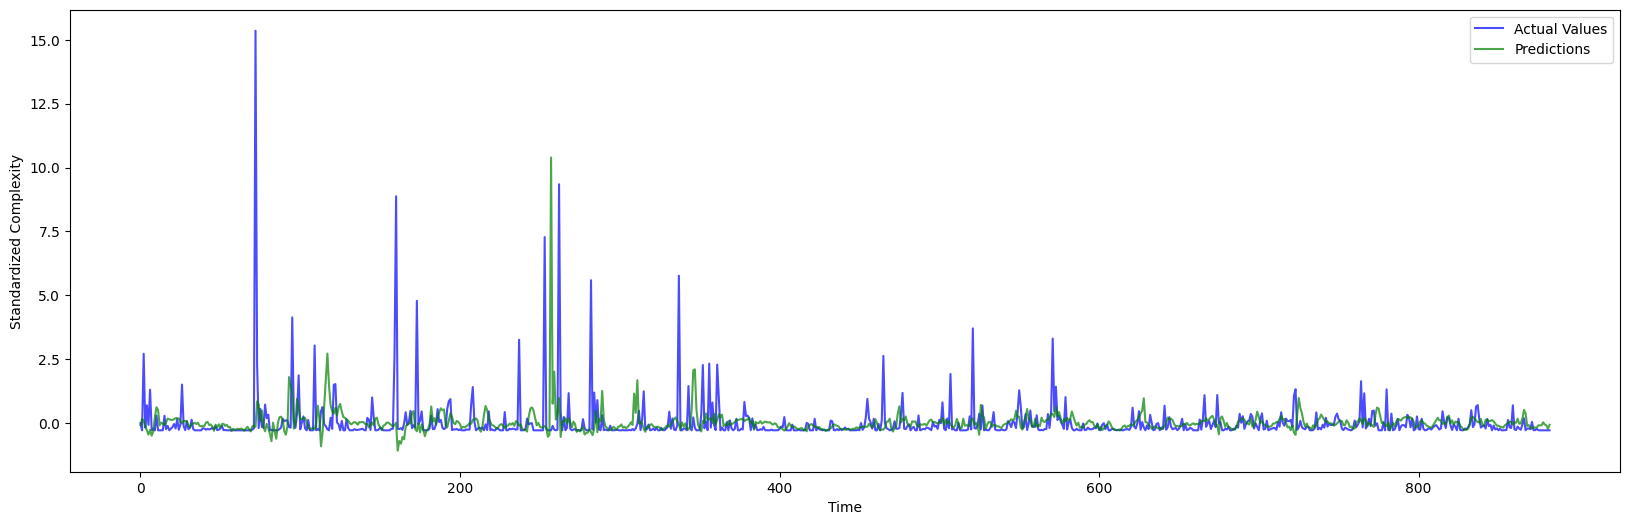
\includegraphics[width=0.9\textwidth]{img/test_accuracy.png}
        \caption{Prediction on the test data}
    \end{figure}
\end{frame}

\subsection{Deep Reinforcement Learning}

\begin{frame}{Deep Reinforcement Learning}
    \begin{itemize}
        \item Environment:
              \begin{itemize}
                  \item total tasks, total nodes
                  \item waiting tasks, available nodes
                  \item executing tasks, executed tasks
              \end{itemize}
        \item Observable states: available nodes, waiting queue (tasks along with waiting times)
        \item Actions: allocating $n \ge 0$ nodes based on available nodes
        \item Algorithms: Actor-Critic \footnotetext{Konda, Vijay, and John Tsitsiklis. "Actor-critic algorithms." Advances in neural information processing systems 12 (1999).} or Proximal Policy Optimization (PPO) \footnotetext{Schulman, John, et al. "Proximal policy optimization algorithms." arXiv preprint arXiv:1707.06347 (2017).}
    \end{itemize}
\end{frame}

\subsection{Comparison}
\begin{frame}
    We compare average waiting times of LSTM scheduler, PPO scheduler against common policies
    \begin{itemize}
        \item Linear scheduler: allocates $\min\{\ell, \texttt{available\_nodes}\}$ for each time stamp, where $\ell$ is a a constant.
        \item Stochastic scheduler: allocates $\min\{x, \texttt{available\_nodes}\}$ for each time stamp, where $x$ is the realization of a random variable $X$ with Poisson distribution.
    \end{itemize}

    LSTM and PPO schedulers take more time to simulate than common policies. For efficiency, PPO performs over two times better than common policies, while LSTM is slightly better.
\end{frame}
\section{Conclusion and Future Work}

\begin{frame}{Conclusion and Future Work}
  \begin{itemize}
    \item RNN and Reinforcement Learning can actually learn something in the scheduling context.
    \item Further experiments can be performed on minutely dataset.
    \item The combinatorial problem when more than one task is submitted at the same time also needs to be studied.
  \end{itemize}
\end{frame}


\begin{frame}{}
    \begin{center}
        \Huge\textbf{Thank you for listening !}
    \end{center}
\end{frame}
% \printbsibliography
\end{document}